\documentclass[11pt]{article}
\usepackage{enumerate}
\usepackage{amsmath}
\usepackage{blindtext}
\usepackage{multicol}
\usepackage{amsfonts}
\usepackage[left=1.5cm,top=2cm,right=1.5cm,bottom=2cm]{geometry}
\usepackage{graphicx}

\newcommand*\varhrulefill[1][0.4pt]{\leavevmode\leaders\hrule height#1\hfill\kern0pt}
\begin{document}

\begin{center}
    \textbf{ITA 1975 - MATEMÁTICA}
\end{center}

\noindent\varhrulefill[0.4mm]

\vspace{6pt}

\noindent \textbf{Notações}

\vspace{6pt}

$\mathbb{N}\quad = \{ 1,2,3, \dots \}$: o conjunto dos números naturais.

$\mathbb{R}\quad$: o conjunto dos números reais.

$\mathbb{C}\quad$: o conjunto dos números complexos.

$i \, \, \quad$: unidade imaginária, $i^2 = -1$.

\vspace{6pt}

\noindent Observação: Os sistemas de coordenadas considerados são os cartesianos retangulares.

\noindent\varhrulefill[0.4mm]

\vspace{12pt}

\parindent0em

\textbf{Questão 1.} Qual é o valor de $\displaystyle \sum_{r=0}^{n} \binom{n}{r}^2$

\begin{multicols}{5}
    \begin{enumerate}[\bf A (\quad)]
        \item $\displaystyle \binom{n}{n}$
        \item $\displaystyle \binom{2n}{n}$
        \item $\displaystyle \binom{n^2}{n}$
        \item $\displaystyle 2^n$
        \item n.d.a.
    \end{enumerate}
\end{multicols}


\textbf{Questão 2.} Seja $\displaystyle f(x) = \frac{e^x - e^{-x}}{e^x + e^{-x}}$ definida em $\mathbb{R}$. Se $g$ for a função inversa de $f$, o valor de $\displaystyle e^{g(7/25)}$ será:

\begin{multicols}{5}
    \begin{enumerate}[\bf A (\quad)]
        \item $\displaystyle \frac{1}{3}$
        \item $\displaystyle \frac{7e}{25}$
        \item $\displaystyle \log_e \left( \frac{25}{7} \right)$
        \item $\displaystyle e^{g(7/25)^2}$
        \item n.d.a.
    \end{enumerate}
\end{multicols}


\textbf{Questão 3.} Uma equação do lugar geométrico das intersecções das diagonais dos retângulos inscritos no triângulo $ABC$ e com um lado em $\overline{AB}$ (figura abaixo) é:

\begin{figure}[h]
    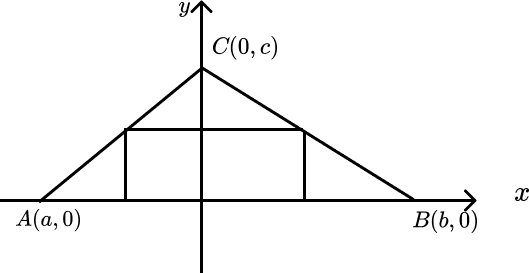
\includegraphics[width=8cm]{./imgs/teste_png.png}
    \centering
\end{figure}

\begin{enumerate}[\bf A (\quad)]
	\item $\displaystyle x + \frac{2(a+b)}{c}y = a + b$
	\item $\displaystyle x - \frac{a+b}{c}y = \frac{a + b}{2}$
	\item $\displaystyle ax + 3(b + c)y = \frac{a + c}{2}$
    \item $x + cy + ab = 0$
    \item n.d.a.
\end{enumerate}

\newpage

\textbf{Questão 4.} A expressão $\displaystyle 1 + \frac{2}{2} + \frac{3}{4} + \frac{4}{8} + \frac{5}{16} + \dots$ vale

\begin{multicols}{5}
    \begin{enumerate}[\bf A (\quad)]
        \item $\displaystyle 4$
        \item $\displaystyle \frac{9}{2}$
        \item $\displaystyle \frac{7}{2}$
        \item $\displaystyle 3,8$
        \item n.d.a.
    \end{enumerate}
\end{multicols}

\textbf{Questão 5.} Se dividirmos um polinômio $P(x)$ por $x-2$ o resto é $13$ e se dividirmos $P(x)$ por $x + 2$ o resto é $5$. Supondo que $R(x)$ é o resto da divisão de $P(x)$ por $x^2 - 4$, podemos afirmar que o valor de $R(X)$, para $x = 1$ é:
 
\begin{multicols}{5}
    \begin{enumerate}[\bf A (\quad)]
        \item $0$
        \item $7$
        \item $9$
        \item $11$
        \item n.d.a.
    \end{enumerate}
\end{multicols}

\textbf{Questão 6.} Seja $A$ uma matriz quadrada de ordem $n$, tal que $A^{-1}=A^t$. Se $\det A = 1$, dizemos que $A$ é uma matriz de rotação, e se $\det A = -1$, $A$ é uma matriz de reflexão. Apoiados em tais definições, podemos afirmar que:

\begin{enumerate}[\bf A (\quad)]
	\item se $n$ é ímpar, o produto de duas matrizes de reflexão é de reflexão.
	\item a soma de duas matrizes de rotação é de rotação.
	\item o produto de duas matrizes de rotação é de rotação.
    \item a matriz inversa de toda matriz de rotação é de reflexão.
    \item n.d.a.
\end{enumerate}

\textbf{Questão 7.} Sabendo-se que $\displaystyle \sin x = \frac{m-n}{m+n}$, $n > 0$ e $m > 0$, podemos afirmar que $\displaystyle \tan \left( \frac{\pi}{4} - \frac{x}{2} \right)$ é igual a

\begin{multicols}{5}
    \begin{enumerate}[\bf A (\quad)]
        \item $\displaystyle \frac{n}{m}$
        \item $\displaystyle \frac{\sqrt{m}}{n}$
        \item $\displaystyle 1 - \frac{n}{m}$
        \item $\displaystyle \sqrt{\frac{n}{m}} $
        \item n.d.a.
    \end{enumerate}
\end{multicols}

\textbf{Questão 8.} A respeito da equação $(x^2 + 3x + 2)^2 - 8(x^2 + 2x) - 8x -1$ podemos afirmar que

\begin{enumerate}[\bf A (\quad)]
    \item todas as raízes são inteiras.
    \item uma raiz é nula e as outras são positivas.
    \item a soma dos módulos das raízes é 6.
    \item o módulo da maior raiz é 5.
    \item n.d.a.
\end{enumerate}

\textbf{Questão 9.} Se $Z_1$, $Z_2$, $Z_3$, $Z_4$ e $Z_5$ são as raízes da equação $(Z + 1)^5 - Z^5 = 0$, e se $R(Z)$ indica a parte real de $Z$ então podemos afirmar que:

\begin{enumerate}[\bf A (\quad)]
    \item $R(Z_K) = 0$ para $K = 1, 2, 3$ e $R(Z_i) = 1$ para $i = 4, 5$.
    \item $\displaystyle R(Z_K) = -\frac{1}{2}$ para $K = 1, 2, 3, 4, 5$.
    \item $Z_1$, $Z_2$, $Z_3$, $Z_4$, $Z_5$ são números reais (não complexos).
    \item $R(Z_K) = 2$ para $K = 1, 2, 3$ e  $R(Z_i) = 0$ para $i = 4, 5$.
    \item n.d.a.
\end{enumerate}

\newpage

\textbf{Questão 10.} Os lados de dois octógonos regulares têm, respectivamente 5 cm e 12 cm. O comprimento do lado de um terceiro octógono regular de área igual à soma das áreas dos outros dois, é:

\begin{multicols}{5}
    \begin{enumerate}[\bf A (\quad)]
        \item 17 cm
        \item 15 cm
        \item 14 cm
        \item 13 cm
        \item n.d.a.
    \end{enumerate}
    \end{multicols}
    

\textbf{Questão 11.} Admitindo-se que o polinômio $P(y) = y^5 - (\tan u)^2 y ^3 + (\tan u) y + \sin^2 u - \tan^2 u$ é divisível pelo polinômio $Q(y) = y + \cot^2 u - \csc^2 u$, onde $\displaystyle \frac{\pi}{2} < u < \pi$, podemos assegurar que:


\begin{enumerate}[\bf A (\quad)]
    \item $\tan u$ é um número irracional negativo.
    \item $\csc u = - \sec u$.
    \item $\displaystyle u = \frac{2\pi}{3}$.
    \item $\tan u$ é um núemro tal que $1 < \tan u < 0$.
    \item n.d.a.
\end{enumerate}


\textbf{Questão 12.} Se $Z_1$ e $Z_2$ são números complexos, $Z_1 + Z_2$ e $Z_1.Z_2$ são ambos reais, então podemos afirmar que 

\begin{enumerate}[\bf A (\quad)]
    \item $Z_1$ e $Z_2$ são ambos reais ou $Z_1 = \overline{Z_2}$.
    \item $Z_1$ e $Z_2$ são números complexos não reais.
    \item $Z_1$ e $Z_2$ são números reais irracionais.
    \item $Z_1$ é um números complexo puro e $Z_2$ é número real.
    \item n.d.a.
\end{enumerate}


\textbf{Questão 13.} Consideremos uma esfera de raio $r = 1$ cm e um ponto $P$ fora desta esfera. Sabendo que a distância deste ponto $P$ à superfície da esfera mede 2 cm. Qual é a razão $K$ entre a área da superfície da esfera e a da calota visível do ponto $P$?

\begin{multicols}{5}
    \begin{enumerate}[\bf A (\quad)]
        \item $K = 1$.
        \item $K = 2$.
        \item $K = 3$.
        \item $\displaystyle K = \frac{5}{2}$.
        \item n.d.a.
    \end{enumerate}
\end{multicols}


\textbf{Questão 14.} Seja $S$ o conjunto das soluções do sistema de desigualdades:

$$
\begin{cases}
2x + y - 3 > 0 \\
x - 2y + 1 < 0 \\
y- 3 < 0 \\
x + my - 5 < 0 
\end{cases}
$$

onde $m$ é real. A representação geométrica de $S$, em coordenadas cartesianas ortogonais $(x,y)$, é:

\begin{enumerate}[\bf A (\quad)]
    \item um quadrilátero para qualquer $m > 0$.
    \item um triângulo isósceles para qualquer $m < 0$.
    \item um triângulo retângulo pata $m < 0$ ou $\displaystyle \frac{5}{3} < m < 4$.
    \item $S$ é o conjunto vazio para $m > \dfrac{5}{3}$.
    \item n.d.a.
\end{enumerate}

\newpage

\textbf{Questão 15.} Sendo $a, b, c, d$ as raízes da equação $2x^4 - 7x^3 + 9x^2 - 7x + 2 = 0$ podemos afirmar que:

\begin{enumerate}[\bf A (\quad)]
    \item $a, b, c, d$ são reais positivas.
    \item $a^2 + b^2 + c^2 + d^2$ é igual a $\dfrac{13}{5}$.
    \item $a, b, c, d$ não são reais.
    \item $\displaystyle \frac{1}{bcd} + \frac{1}{acd} + \frac{1}{abd} + \frac{1}{abc}$ é a soma das raízes.
    \item n.d.a.
\end{enumerate}

\textbf{Questão 16.} As medidas dos catetos de um triângulo retângulo são $(\sin x)$ cm e $(\cos x)$ cm. Um estudante calculou o volume do sólido gerado pela rotação deste triângulo em torno da hipotenusa e obteve como resultado $\pi$ cm$^3$. Considere este resultado como certo, podemos afirmar que:

\begin{multicols}{5}
    \begin{enumerate}[\bf A (\quad)]
        \item $x = \dfrac{\pi}{6}$
        \item $x = \dfrac{\pi}{3}$
        \item $x = \dfrac{\pi}{4}$
        \item $x = \dfrac{\pi}{5}$
        \item n.d.a.
    \end{enumerate}
\end{multicols}

\textbf{Questão 17.} Sejam as matrizes reais $A = \begin{bmatrix} a & b \\ c & d \end{bmatrix}$, $I = \begin{bmatrix} 1 & 0 \\ 0 & 1 \end{bmatrix}$, $X = \begin{bmatrix} x \\ y \end{bmatrix}$ e $m$ um número real. Seja: $AX = mX$, Então podemos afirmar que: 

\begin{enumerate}[\bf A (\quad)]
    \item Se $\det (A - mI) \neq 0$, então $x + y = 0$ e $x.y \neq 0$.
    \item Se $\det (A - mI) = 0$, então existem dois números reais $x, y$ tais que $x + y \neq 0$ ou $x.y \neq 0$.
    \item Se $\det (A - mI) = 0$, então $\det A = 0$ e $m = 0$.
    \item Se $\det A = 0$, então não existem dois números reais $x, y$ tais que $AX = mX$.
    \item n.d.a.
\end{enumerate}

\textbf{Questão 18.} As dimissões de um paralelepípedo retângulo são proporcionais aos números $\log_e t$, $\log_e t^2$, $\log_e t^3$ e a área total é 792 cm$^2$. Sabendo-se que a soma das dimenssões vale 12 vezes a razão de proporcionalidade. Quais são os valores destas dimenssões?

\begin{multicols}{5}
    \begin{enumerate}[\bf A (\quad)]
        \item 6, 12 e 18.
        \item 5, 10 e 15.
        \item 2, 3 e 4.
        \item 2, 4 e 8.
        \item n.d.a.
    \end{enumerate}
\end{multicols}

\textbf{Questão 19.} O número de soluções inteiras e não negativas da equação $x + y + z + 1 = 7 $ é:

\begin{multicols}{5}
    \begin{enumerate}[\bf A (\quad)]
        \item $\displaystyle \binom{7}{4}$
        \item $\displaystyle \binom{11}{4}$
        \item $\displaystyle \binom{10}{3}$
        \item $\displaystyle \binom{11}{3}$
        \item n.d.a.
    \end{enumerate}
\end{multicols}

\textbf{Questão 20.} Seja $ABCD$ um quadrilátero convexo inscrito em uma circunferência. Sabe-se que $\hat{A} = 2\hat{C}$, $\hat{B} > \hat{D}$ e $\tan \hat{B}.\tan \hat{D} + \sin \hat{A}. \sin \hat{C} = -\dfrac{9}{4}$. Neste caso, os valores de $\hat{A}, \hat{B}, \hat{C}, \hat{D}$ são respectivamente:

\begin{multicols}{3}
    \begin{enumerate}[\bf A (\quad)]
        \item $150^{\circ}$, $45^{\circ}$, $75^{\circ}$, $30^{\circ}$
        \item $90^{\circ}$, $120^{\circ}$, $45^{\circ}$, $60^{\circ}$
        \item $120^{\circ}$, $150^{\circ}$, $60^{\circ}$, $30^{\circ}$
        \item $120^{\circ}$, $120^{\circ}$, $60^{\circ}$, $60^{\circ}$
        \item n.d.a.
    \end{enumerate}
\end{multicols}

\newpage

\textbf{Questão 21.} Num triângulo escaleno $ABC$, os lados opostos aos ângulos $A, B, C$ medem, respectivamente, $a, b ,c$. Então a expressão: $a \sin(\hat{B} - \hat{C}) + b \sin(\hat{C} - \hat{A}) +  c \sin(\hat{A} - \hat{B})$


\begin{multicols}{3}
    \begin{enumerate}[\bf A (\quad)]
        \item $a\sin\hat{A}+b\sin\hat{B}+c\sin\hat{C}$.
        \item $\sin^2\hat{A}+\sin^2\hat{B}+\sin^2\hat{C}$.
        \item 0.
        \item 1.
        \item n.d.a.
    \end{enumerate}
\end{multicols}

\textbf{Questão 22.} Considere a circunferência $C$ que pelos pontos $(0,0)$, $(2,0)$ e $(0,2)$ em um sistema de coordenadas cartesianas ortogonais. Uma das retas tangentes a esta circunferência, que passa pelo ponto $(3,5)$, tem por equação

\begin{multicols}{3}
\begin{enumerate}[\bf A (\quad)]
    \item $x + y - 3 = 0$.
    \item $7x - y + 8 = 0$.
    \item $x - y + 2 = 0$.
    \item $6x - y - 16 = 0$
    \item n.d.a.
\end{enumerate}
\end{multicols}

\textbf{Questão 23.} Se, na figura abaixo, $c$ é uma circunferência de raio $R$, $r$ e $s$ são retas tangentes à circunferência e $\overline{OT} = 2R$ então o ângulo $\alpha$ das retas $r$ e $s$ deve verificar uma das alternativas seguintes:

\begin{figure}[h]
    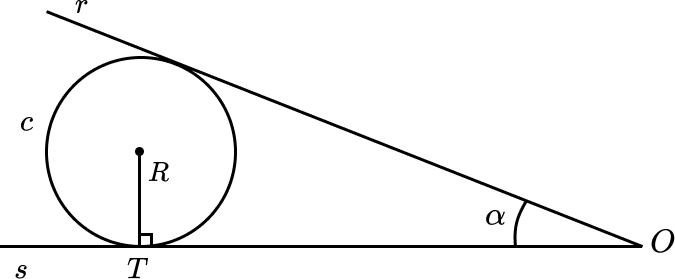
\includegraphics[width=8cm]{./imgs/figure_ita_1975_matematica_q23.png}
    \centering
\end{figure}

\begin{multicols}{3}
    \begin{enumerate}[\bf A (\quad)]
        \item $\sin \alpha = \dfrac{4}{5}$ e $\cos \alpha = \dfrac{3}{5}$
        \item $\cos \alpha = \dfrac{4}{5}$ e $\sin \alpha = \dfrac{3}{5}$
        \item $\sin \alpha = \dfrac{\sqrt{3}}{2}$ e $\cos \alpha = \dfrac{1}{2}$
        \item $\cos \alpha = \dfrac{\sqrt{3}}{2}$ e $\sin \alpha = \dfrac{1}{2}$
        \item n.d.a.
    \end{enumerate}
\end{multicols}

\textbf{Questão 24.} A respeito da equação exponencial $4^x + 6^x = 9^x$ podemos afirmar que:

\begin{enumerate}[\bf A (\quad)]
    \item $\displaystyle x = 9 \log_{10} \left(\frac{1 + \sqrt{3}}{2}\right)$ é uma raiz.
    \item $\displaystyle x = \left[\log_{10}\left(\frac{3}{2}\right)\right]^{-1}.\log_{10}\left(\frac{1 + \sqrt{5}}{2}\right)$ é uma raiz. 
    \item $\displaystyle x = \left[\log_{10}\left(\frac{3}{2}\right)\right]^{-1}.\log_{10}\left(\frac{1 + \sqrt{3}}{2}\right)$ é uma raiz. 
    \item $\displaystyle x = \left[\log_{10}\left(\frac{3}{2}\right)\right]^{-1}.\log_{10}\left(\frac{1 + \sqrt{6}}{2}\right)$ é uma raiz. 
    \item n.d.a.
\end{enumerate}

\newpage

\textbf{Questão 25.} Seja $S = \log_3(\tan x_1) + \log_3(\tan x_2) + \log_3(\tan x_3) + \dots$ onde $x_1 = \dfrac{\pi}{3}$ e $x_{n+1} = \arctan(\sqrt{\tan x_n})$, $n = 2, 3, \dots$.


    \begin{enumerate}[\bf A (\quad)]
        \item $S = \log_3 (\tan x_1 + \tan x_2 + \tan x_1 + \dots)$.
        \item $S = -1$
        \item $S = 2$
        \item $S = 1$
        \item n.d.a.
    \end{enumerate}

\end{document}